\documentclass[a4paper, 14pt]{extarticle}

% Поля
%--------------------------------------
\usepackage{geometry}
\geometry{a4paper,tmargin=2cm,bmargin=2cm,lmargin=3cm,rmargin=1cm}
%--------------------------------------


%Russian-specific packages
%--------------------------------------
\usepackage[T2A]{fontenc}
\usepackage[utf8]{inputenc} 
\usepackage[english, main=russian]{babel}
%--------------------------------------

\usepackage{textcomp}

% Красная строка
%--------------------------------------
\usepackage{indentfirst}               
%--------------------------------------             


%Graphics
%--------------------------------------
\usepackage{graphicx}
\graphicspath{ {./images/} }
\usepackage{wrapfig}
%--------------------------------------

% Полуторный интервал
%--------------------------------------
\linespread{1.3}                    
%--------------------------------------

%Выравнивание и переносы
%--------------------------------------
% Избавляемся от переполнений
\sloppy
% Запрещаем разрыв страницы после первой строки абзаца
\clubpenalty=10000
% Запрещаем разрыв страницы после последней строки абзаца
\widowpenalty=10000
%--------------------------------------

%Списки
\usepackage{enumitem}

%Подписи
\usepackage{caption} 

%Гиперссылки
\usepackage{hyperref}

\hypersetup {
	unicode=true
}

%Рисунки
%--------------------------------------
\DeclareCaptionLabelSeparator*{emdash}{~--- }
\captionsetup[figure]{labelsep=emdash,font=onehalfspacing,position=bottom}
%--------------------------------------

\usepackage{tempora}

%Листинги
%--------------------------------------
\usepackage{listings}
\lstset{
  basicstyle=\ttfamily\footnotesize, 
  %basicstyle=\footnotesize\AnkaCoder,        % the size of the fonts that are used for the code
  breakatwhitespace=false,         % sets if automatic breaks shoulbd only happen at whitespace
  breaklines=true,                 % sets automatic line breaking
  captionpos=t,                    % sets the caption-position to bottom
  inputencoding=utf8,
  frame=single,                    % adds a frame around the code
  keepspaces=true,                 % keeps spaces in text, useful for keeping indentation of code (possibly needs columns=flexible)
  keywordstyle=\bf,       % keyword style
  numbers=left,                    % where to put the line-numbers; possible values are (none, left, right)
  numbersep=5pt,                   % how far the line-numbers are from the code
  xleftmargin=25pt,
  xrightmargin=25pt,
  showspaces=false,                % show spaces everywhere adding particular underscores; it overrides 'showstringspaces'
  showstringspaces=false,          % underline spaces within strings only
  showtabs=false,                  % show tabs within strings adding particular underscores
  stepnumber=1,                    % the step between two line-numbers. If it's 1, each line will be numbered
  tabsize=2,                       % sets default tabsize to 8 spaces
  title=\lstname                   % show the filename of files included with \lstinputlisting; also try caption instead of title
}
%--------------------------------------

%%% Математические пакеты %%%
%--------------------------------------
\usepackage{amsthm,amsfonts,amsmath,amssymb,amscd}  % Математические дополнения от AMS
\usepackage{mathtools}                              % Добавляет окружение multlined
\usepackage[perpage]{footmisc}
%--------------------------------------

%--------------------------------------
%			НАЧАЛО ДОКУМЕНТА
%--------------------------------------

\begin{document}

%--------------------------------------
%			ТИТУЛЬНЫЙ ЛИСТ
%--------------------------------------
\begin{titlepage}
\thispagestyle{empty}
\newpage


%Шапка титульного листа
%--------------------------------------
\vspace*{-60pt}
\hspace{-65pt}
\begin{minipage}{0.3\textwidth}
\hspace*{-20pt}\centering

\includegraphics[width=\textwidth]{emblem}
\end{minipage}
\begin{minipage}{0.67\textwidth}\small \textbf{
\vspace*{-0.7ex}
\hspace*{-6pt}\centerline{Министерство науки и высшего образования Российской Федерации}
\vspace*{-0.7ex}
\centerline{Федеральное государственное бюджетное образовательное учреждение }
\vspace*{-0.7ex}
\centerline{высшего образования}
\vspace*{-0.7ex}
\centerline{<<Московский государственный технический университет}
\vspace*{-0.7ex}
\centerline{имени Н.Э. Баумана}
\vspace*{-0.7ex}
\centerline{(национальный исследовательский университет)>>}
\vspace*{-0.7ex}
\centerline{(МГТУ им. Н.Э. Баумана)}}
\end{minipage}
%--------------------------------------

%Полосы
%--------------------------------------
\vspace{-25pt}
\hspace{-35pt}\rule{\textwidth}{2.3pt}

\vspace*{-20.3pt}
\hspace{-35pt}\rule{\textwidth}{0.4pt}
%--------------------------------------

\vspace{1.5ex}
\hspace{-35pt} \noindent \small ФАКУЛЬТЕТ\hspace{80pt} <<Информатика и системы управления>>

\vspace*{-16pt}
\hspace{47pt}\rule{0.83\textwidth}{0.4pt}

\vspace{0.5ex}
\hspace{-35pt} \noindent \small КАФЕДРА\hspace{50pt} <<Теоретическая информатика и компьютерные технологии>>

\vspace*{-16pt}
\hspace{30pt}\rule{0.866\textwidth}{0.4pt}
  
\vspace{11em}

\begin{center}
\Large {\bf Лабораторная работа № 1} \\ 
\large {\bf по курсу <<Методы оптимизации>>} \\
\large <<Поиск минимума унимодальной функции>> 
\end{center}\normalsize

\vspace{8em}


\begin{flushright}
  {Студент группы ИУ9-82Б Виленский С. Д. \hspace*{15pt}\\ 
  \vspace{2ex}
  Преподаватель Посевин Д. П.\hspace*{15pt}}
\end{flushright}

\bigskip

\vfill
 

\begin{center}
\textsl{Москва 2024}
\end{center}
\end{titlepage}
%--------------------------------------
%		КОНЕЦ ТИТУЛЬНОГО ЛИСТА
%--------------------------------------

\renewcommand{\ttdefault}{pcr}

\setlength{\tabcolsep}{3pt}
\newpage
\setcounter{page}{2}

\section{Задание}\label{Sect::task}

Определить интервал, на котором функция является унимодальной, алгоритм 
определения унимодальности должен принимать на вход левую и правую точку 
отрезка и возвращать false — если функция на этом отрезке не унимодальная, в 
противном случае true.  
Реализовать поиск минимума унимодальной функции на полученном 
интервале методом прямого перебора, дихотомии (деление отрезка пополам), 
золотого сечения и Фибоначчи с заданной точностью по вариантам. Результат 
должен быть представлен на графике, точки минимизирующей последовательности должны быть выделены красным цветом, интервалы деления синим. 
Точность вычисления точки минимума должна варьироваться. 

\section{Результаты}\label{Sect::res}

Исходный код программы представлен в листингах~\ref{lst:code1}-~\ref{lst:code4}.

\begin{figure}[!htb]
\begin{lstlisting}[language={},caption={Нахождение минимумов функции},label={lst:code1}]
using Plots

function derivativeAtPoint(f, x)
    delta = 1e-3
    return (f(x + delta) - f(x)) / delta
end

function secondDerivativeAtPoint(f, x)
    delta = 1e-3
    return (derivativeAtPoint(f, x + delta) - derivativeAtPoint(f, x)) / delta
end

function findUnimodalIntervals(f, a, b, step)
    intervals = []
    actual_interval_start = a
    
    for x in a:step:b
        if secondDerivativeAtPoint(f, x) <= 0
            if abs(actual_interval_start - x) > step * 2
                push!(intervals, (actual_interval_start, x))
            end
            actual_interval_start = x
        end
    end
    if abs(actual_interval_start - b) > step * 2
        push!(intervals, (actual_interval_start, b))
    end
\end{lstlisting}
\end{figure}
\begin{figure}[!htb]
\begin{lstlisting}[language={},caption={Нахождение минимумов функции},label={lst:code2}]
    return intervals
end

function findExtrBySegments(f, a, b, step, eps)
    iters = []

    while abs(a - b) > eps
        x1 = a + (b - a) / 3
        x2 = a + (b - a) * 2 / 3

        push!(iters, (a, x1, x2, b))

        if f(x1) > f(x2)
            a = x1
        else
            b = x2
        end
    end

    return (a + b) / 2, iters
end

function findExtrByGoldRatio(f, a, b, step, eps)
    iters = []

    goldRatio = (5^.5 - 1) / 2
    x1 = a + (1 - goldRatio) * (b - a)
    x2 = a + goldRatio * (b - a)
    x = (a + b) / 2

    while abs(a - b) > eps
        push!(iters, (a, x1, x2, b))

        if f(x1) > f(x2)
            x = x2
            a = x1
            x1 = x2
            x2 = a + b - x2
        else
            x = x1
            b = x2
            x2 = x1
            x1 = a + b - x1
        end
    end

    return x, iters
end

function findExtrByFibbonachi(f, a, b, step, eps)
    iters = []

    fib1, fib2, fib3 = 0, 1, 1
    for i in 1:16
\end{lstlisting}
\end{figure}
\begin{figure}[!htb]
\begin{lstlisting}[language={},caption={Нахождение минимумов функции},label={lst:code3}]

        fib1 = fib2
        fib2 = fib3
        fib3 = fib1 + fib2
    end
    x1 = a + (fib1 / fib3) * (b - a)
    x2 = a + b - x1
    x = (a + b) / 2

    while abs(a - b) > eps
        push!(iters, (a, x1, x2, b))

        if f(x1) > f(x2)
            x = x2
            a = x1
            x1 = x2
            x2 = a + b - x2
        else
            x = x1
            b = x2
            x2 = x1
            x1 = a + b - x1
        end
    end

    return x, iters
end

f = x -> x ^ 4 - 2 * x ^ 2 + 3

intervals = findUnimodalIntervals(f, -10, 10, 2e-6)

interval_index = 1
a = intervals[interval_index][1]
b = intervals[interval_index][2]
alg_step = 2e-3
alg_eps = 1e-3

X = range(a, b, step=alg_step)
Y = [f(x) for x in X]
Y_min = minimum(Y)
Y_max = maximum(Y)
prop_Y = c -> Y_max - (Y_max - Y_min) * c

plot(X, Y, legend=false, title="ExtrBySegments")

x0, iters = findExtrBySegments(f, a, b, alg_step, alg_eps)
println(length(iters))
for (i, iter) in enumerate(iters)
    y_val = prop_Y(i / length(iters))

    hline!([y_val], color="green")
    scatter!([(iter[2], y_val), (iter[3], y_val)], color="blue")
    scatter!([(iter[1], y_val), (iter[4], y_val)], color="red")
end
\end{lstlisting}
\end{figure}
\begin{figure}[!htb]
\begin{lstlisting}[language={},caption={Нахождение минимумов функции},label={lst:code4}]

plot!()

X = range(a, b, step=alg_step)
Y = [f(x) for x in X]
Y_min = minimum(Y)
Y_max = maximum(Y)
prop_Y = c -> Y_max - (Y_max - Y_min) * c

plot(X, Y, legend=false, title="ExtrByGoldRatio")

x0, iters = findExtrByGoldRatio(f, a, b, alg_step, alg_eps)
println(length(iters))
for (i, iter) in enumerate(iters)
    y_val = prop_Y(i / length(iters))

    hline!([y_val], color="green")
    scatter!([(iter[2], y_val), (iter[3], y_val)], color="blue")
    scatter!([(iter[1], y_val), (iter[4], y_val)], color="red")
end

plot!()

X = range(a, b, step=alg_step)
Y = [f(x) for x in X]
Y_min = minimum(Y)
Y_max = maximum(Y)
prop_Y = c -> Y_max - (Y_max - Y_min) * c

plot(X, Y, legend=false, title="ExtrByFibbonachi")

x0, iters = findExtrByFibbonachi(f, a, b, alg_step, alg_eps)
println(length(iters))
for (i, iter) in enumerate(iters)
    y_val = prop_Y(i / length(iters))

    hline!([y_val], color="green")
    scatter!([(iter[2], y_val), (iter[3], y_val)], color="blue")
    scatter!([(iter[1], y_val), (iter[4], y_val)], color="red")
end

plot!()
\end{lstlisting}
\end{figure}

Результат запуска представлен в листинге ~\ref{lst:res1} и рисунках ~\ref{fig:img1}-~\ref{fig:img3}.

\begin{figure}[!htb]
\begin{lstlisting}[language={},caption={Нахождение минимумов функции},label={lst:res1}]
(-10, -0.57835)
(0.57635, 10)

ExtrBySegments - 23
ExtrByGoldRatio - 20
ExtrByFibbonachi - 18
\end{lstlisting}
\end{figure}

\begin{figure}[!htb]
	\centering
	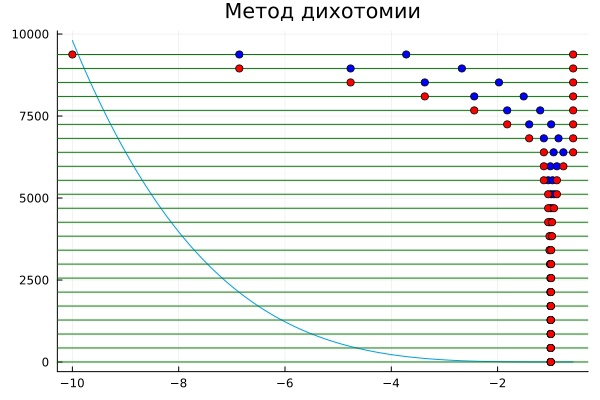
\includegraphics[width=0.8\textwidth]{img1}
\caption{Результат работы алгоритма методом дихотомии}
\label{fig:img1}
\end{figure}


\begin{figure}[!htb]
	\centering
	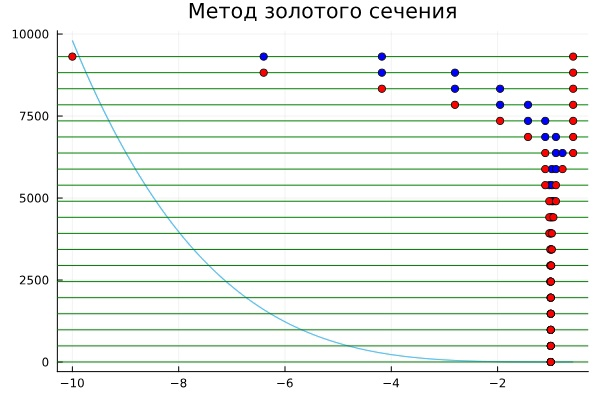
\includegraphics[width=0.8\textwidth]{img2}
\caption{Результат работы алгоритма методом золотого сечения}
\label{fig:img2}
\end{figure}


\begin{figure}[!htb]
	\centering
	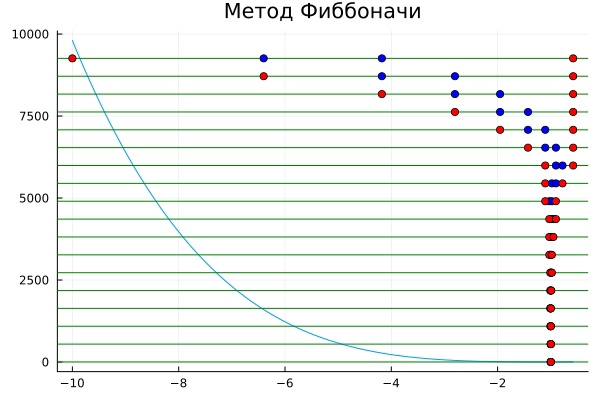
\includegraphics[width=0.8\textwidth]{img3}
\caption{Результат работы алгоритма методом Фиббоначи}
\label{fig:img3}
\end{figure}

\section{Выводы}\label{Sect::task}

 Исходя из результатов исследования можно сделать вывод о том, что метод Фибоначи является в данном случае наиболее подходящим, судя по скорости сходимости алгоритма, в то время как метод золотого сечения показал себя лучше метода схлодящимися отрезками, также известного как метод Дихотомии.

\end{document}
